\marginnote{\hfill \Chapref{chap:pstask} \adforn{43}}

% =======================================================

\section{Context}
\label{sec:overview:context}

Welcome to this thesis template :) You can use it as you want: you are not obliged to mention this template, but it would be nice to do so (e.g., keep the colophon). 

% =======================================================

\section{Main contributions}
\label{sec:overview:contributions}

This dissertation aims to …. To that end, we design two algorithms:

% -------------------------------------------------------

\subsection{First part name}

MTH1 introduction …

Our contribution includes:
\blinditemize[2]

\newthought{} In the rest of this dissertation, we refer to this method as MTH1.

% -------------------------------------------------------

\subsection{Second part name}

Idem

% -------------------------------------------------------

\subsection{Other contributions}

Our other contribution includes:
\blinditemize[2]

% =======================================================

\section{Organization of the dissertation}
\label{sec:overview:organization}

\begin{description}
    \item Chapter \ref{chap:task} presents some typography tips.
\end{description}

\newthought{} The rest of the dissertation is composed of the two proposed approaches:

\paragraph{Part name}
\begin{description}
    \item Chapter \ref{chap:sota1} is an example of state of the art chapter.
    \item Chapter \ref{chap:mth1} describes the equation and algorithms.
    \item Chapter \ref{chap:res1} walks through figures and tables.
\end{description}

\paragraph{Part name}
\begin{description}
    \item Chapter \ref{chap:sota2} presents an empty state of the art.
\end{description}

Finally, the dissertation concludes with Chapter \ref{chap:conclusion}, which summarizes the contributions and suggests a few additional research ideas.

\paragraph{General appendices}
\begin{description}
    \item Appendix \ref{chap:61} is an introduction to deep learning.
\end{description}

\vfill

\begin{plate*}
    \centering
    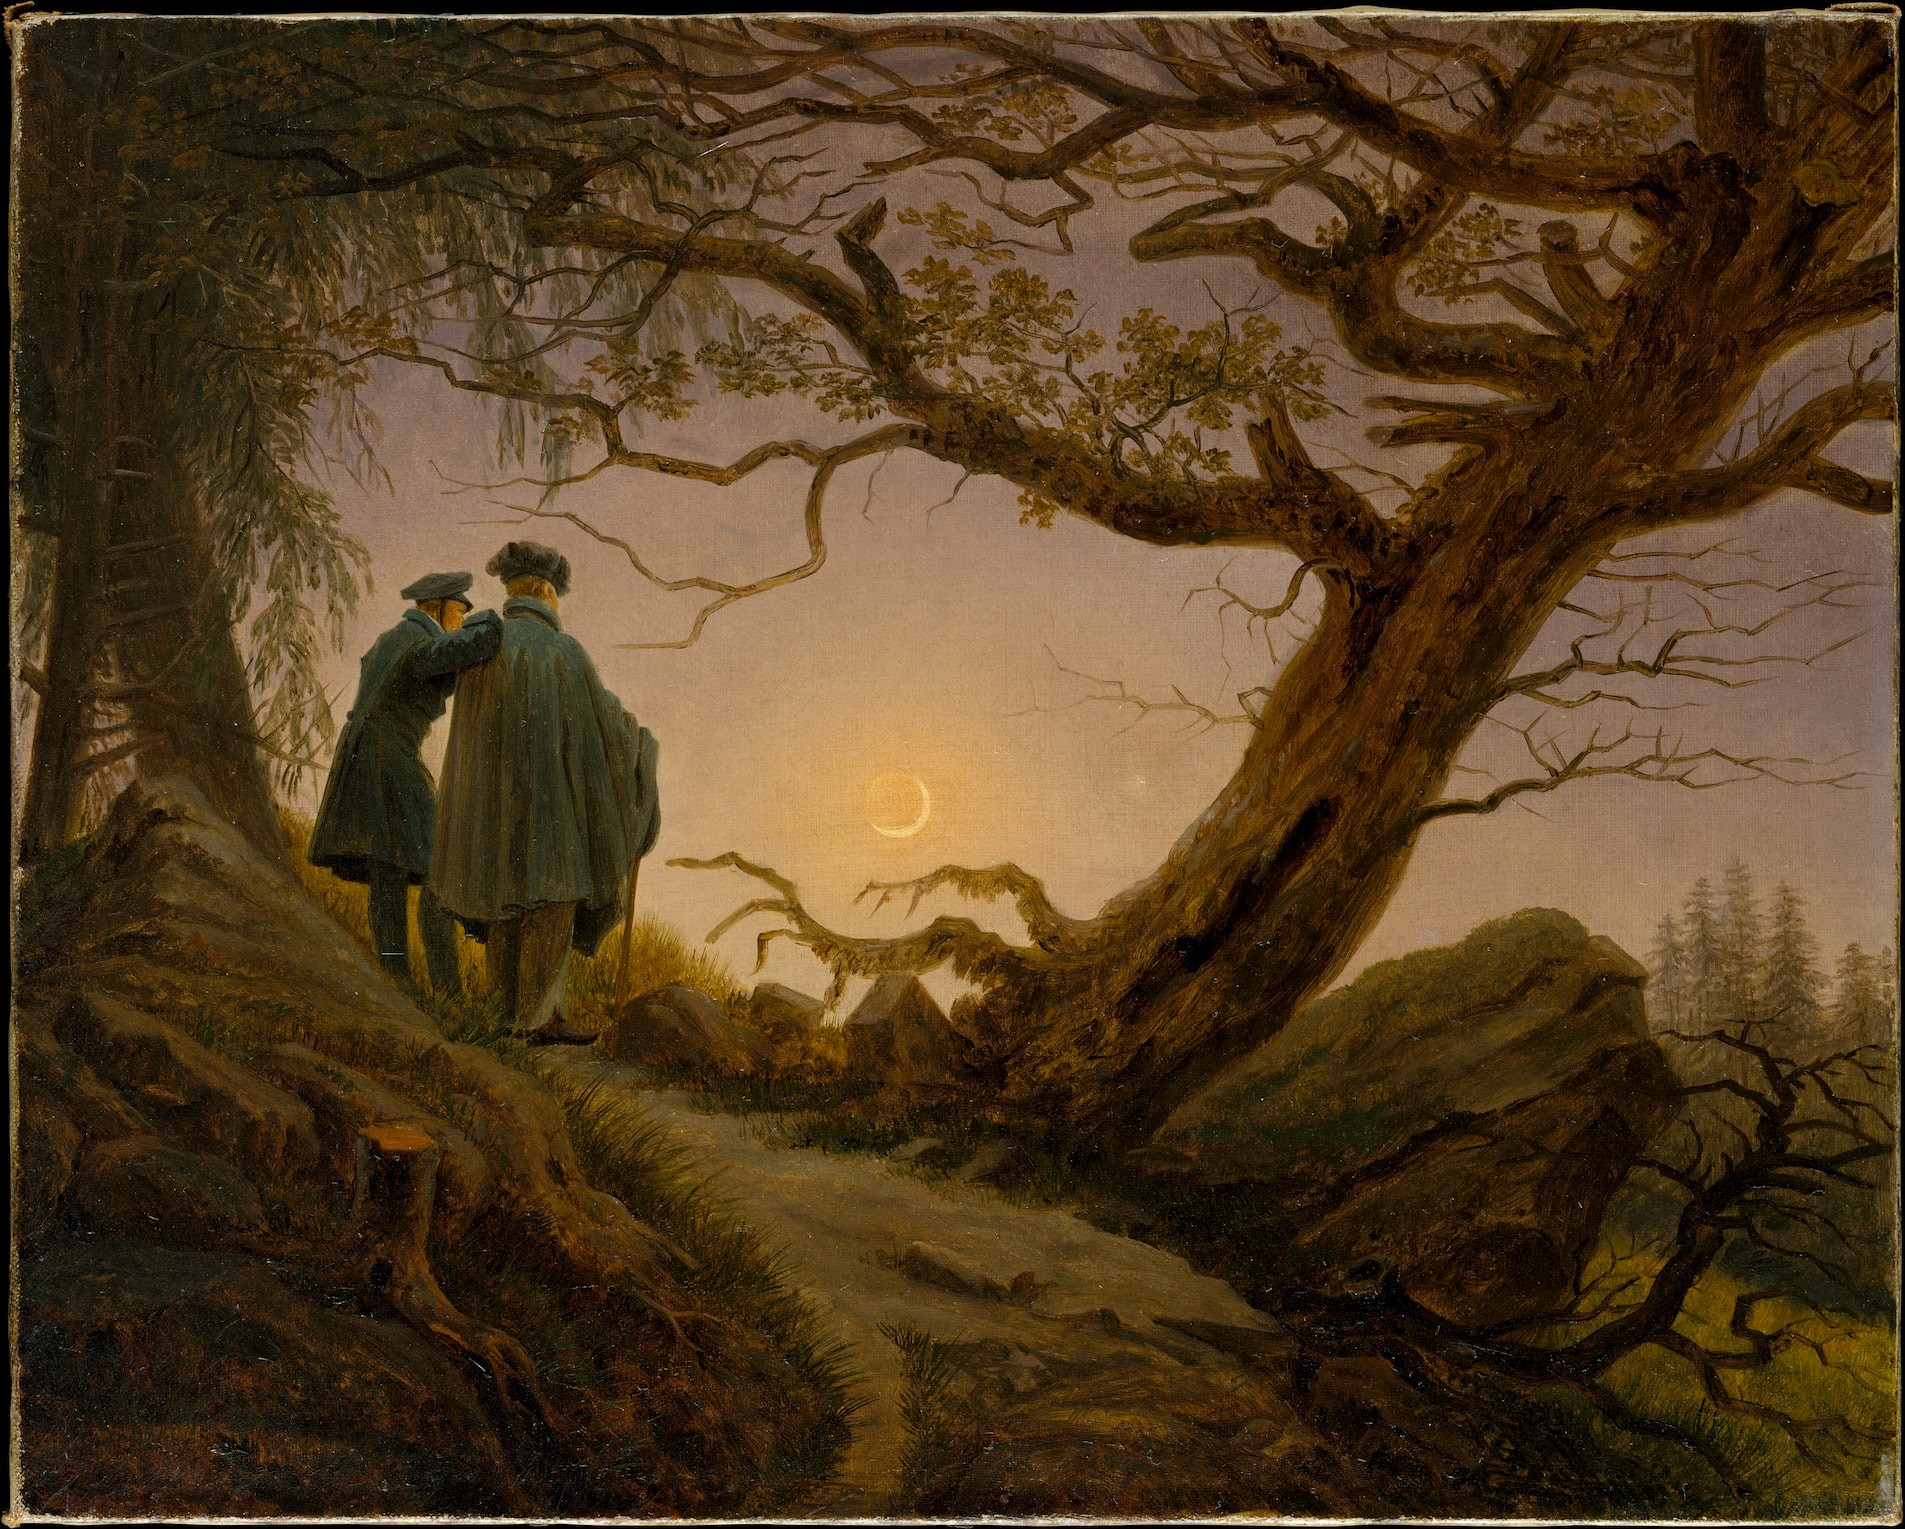
\includegraphics[width=\textwidth]{00-met-artwork/friedrich_moon.jpg}
    \caption[Two Men Contemplating the Moon, Caspar David Friedrich]{\href{https://www.metmuseum.org/art/collection/search/438417}{\textit{Two Men Contemplating the Moon}}, Caspar David Friedrich, ca. 1825-30, from the  MET Open Collections.}
\end{plate*}